\documentclass[../main]{subfiles}
\usetikzlibrary{arrows.meta,decorations.markings,calc,patterns}

\begin{document}

\chapter{Cavitación}

\section{Cavitación}

\subsection{Introducción a la cavitación}

La cavitación es un fenómeno que ocurre en los líquidos cuando estos son sometidos a una reducción de presión tan grande que se forman burbujas de vapor en su interior. Estas burbujas pueden colapsar violentamente, causando daños en superficies cercanas. La cavitación es un problema común en bombas, hélices y turbinas hidráulicas.

\info{Definición de cavitación}{
La cavitación se produce cuando la presión local en un fluido baja por debajo de su presión de vapor\footnote{Presión de vapor: la presión a la cual un líquido comienza a convertirse en vapor a una temperatura dada.}, permitiendo que se formen burbujas de vapor.
}

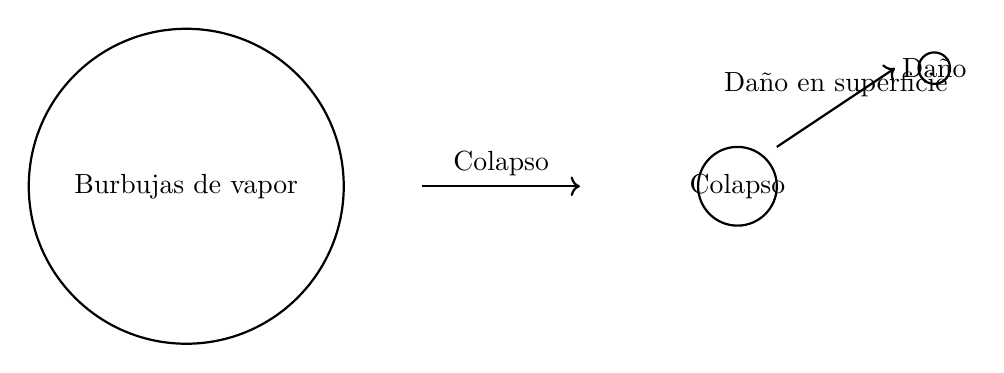
\begin{tikzpicture}
    \draw[thick] (0,0) circle (2);
    \node at (0,0) {Burbujas de vapor};
    \draw[->,thick] (3,0) -- (5,0) node[midway,above] {Colapso};
    \draw[thick] (7,0) circle (0.5);
    \node at (7,0) {Colapso};
    \draw[->,thick] (7.5,0.5) -- (9,1.5) node[midway,above] {Daño en superficie};
    \draw[thick] (9.5,1.5) circle (0.2);
    \node at (9.5,1.5) {Daño};
\end{tikzpicture}

\info{Formación de burbujas}{
Las burbujas de cavitación se forman en regiones donde la presión del líquido cae por debajo de la presión de vapor del líquido. 
}

\subsection{Ecuaciones Relacionadas con la Cavitación}

La cavitación se puede analizar utilizando varias ecuaciones clave, que describen el comportamiento del fluido y la formación de burbujas.

\info{Ecuación de Bernoulli}{
La ecuación de Bernoulli para un fluido incompresible y sin viscosidad es:
\begin{equation}
P + \frac{1}{2} \rho v^2 + \rho gh = \text{constante}
\end{equation}
Siendo:
\begin{itemize}
    \item $P$: Presión del fluido [Pa]
    \item $\rho$: Densidad del fluido [kg/m^3]
    \item $v$: Velocidad del fluido [m/s]
    \item $g$: Aceleración debida a la gravedad [m/s^2]
    \item $h$: Altura [m]
\end{itemize}
}

\info{Número de cavitación}{
El número de cavitación $C_v$ es una medida adimensional utilizada para predecir la formación de cavitación y está dado por:
\begin{equation}
C_v = \frac{P - P_v}{\frac{1}{2} \rho v^2}
\end{equation}
Siendo:
\begin{itemize}
    \item $P$: Presión del líquido [Pa]
    \item $P_v$: Presión de vapor del líquido [Pa]
    \item $\rho$: Densidad del líquido [kg/m^3]
    \item $v$: Velocidad del líquido [m/s]
\end{itemize}
}

\info{Tensión superficial y radio de burbuja}{
La relación entre la tensión superficial y el radio de una burbuja está dada por la ecuación de Young-Laplace:
\begin{equation}
\Delta P = \frac{2 \sigma}{R}
\end{equation}
Siendo:
\begin{itemize}
    \item $\Delta P$: Diferencia de presión entre el interior y el exterior de la burbuja [Pa]
    \item $\sigma$: Tensión superficial del líquido [N/m]
    \item $R$: Radio de la burbuja [m]
\end{itemize}
}

\ejemplo{Ejemplo de cavitación en una bomba}{
Supongamos una bomba que impulsa agua a una velocidad de $10 \, \text{m/s}$ y que la presión en el punto más bajo de la bomba es de $50000 \, \text{Pa}$. La densidad del agua es $1000 \, \text{kg/m}^3$ y la presión de vapor del agua a la temperatura de operación es de $2500 \, \text{Pa}$. Calcular el número de cavitación.

Datos:
\begin{itemize}
    \item $P = 50000 \, \text{Pa}$
    \item $P_v = 2500 \, \text{Pa}$
    \item $\rho = 1000 \, \text{kg/m}^3$
    \item $v = 10 \, \text{m/s}$
\end{itemize}

\begin{equation}
C_v = \frac{P - P_v}{\frac{1}{2} \rho v^2} = \frac{50000 - 2500}{\frac{1}{2} \times 1000 \times 10^2} = \frac{47500}{50000} = 0.95
\end{equation}
}

\actividad{Responder el siguiente cuestionario}
\begin{enumerate}
\item ¿Qué es la cavitación?
\item ¿En qué condiciones se produce la cavitación?
\item ¿Qué daños puede causar la cavitación?
\item ¿Cómo se relaciona la presión de vapor con la cavitación?
\item ¿Qué es el número de cavitación?
\item ¿Cómo afecta la velocidad del fluido a la cavitación?
\item ¿Qué papel juega la ecuación de Bernoulli en la cavitación?
\item ¿Cómo se puede prevenir la cavitación en una bomba?
\item ¿Qué es la tensión superficial y cómo se relaciona con las burbujas de cavitación?
\item ¿Qué factores afectan la presión de vapor de un líquido?
\end{enumerate}

\end{document}
